
\section{Introduction}
\label{sec-introduction}

Finding the optimal Binary Search Tree (BST) is a somewhat classical programming problem. Given a set of keys and a probability that each key will be looked up i.e. frequency, the optimal BST is structured s.t. the expected search time over all keys is minimized. The expected cost of searching for any arbitrary key is $frequency \times (depth + 1)$. The expected search time of the entire BST is simply the sum of the search costs of all keys. Specifically, the goal is to construct a BST that minimizes the expected search time, while maintaining BST properties given the key values. Thus, it is preferable to have keys with higher frequencies at a shorter depth. Figure~\ref{fig:opt-bst} shows 5 different BSTs that can be constructed given a set of keys (value row).

\begin{figure}[h]
    \centering
    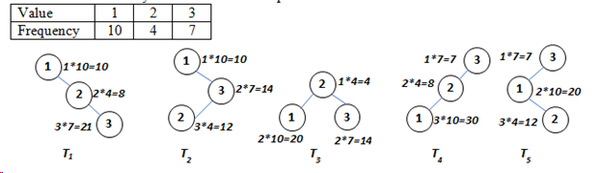
\includegraphics[width=0.9\columnwidth]{figures/opt_bst.png}
    \caption{ \small Various BST structures constructed from the same keys (reproduced from~\cite{bst_figure}).}
    \label{fig:opt-bst}
\end{figure}

A solution to the optimal BST problem is to simply try each key as root and recursively build each subtree. After exhaustively constructing every valid BST structure, the one with the minimum cost can be chosen. Given a tree with $n$ nodes, this would take exponential time to solve. However, this naive solution can be further improved to $O(n^3)$ with dynamic programming. Although finding the optimal BST structure for any arbitrary set of keys and frequencies has been bounded, we would like to explore the application of an evolutionary algorithm to this problem.

\subsection{Problem Statement}

Given a set of keys $k_1,k_2,\dots,k_n$ and a set of frequencies $f_1,f_2,\dots,f_n$ s.t. $f_i$ is the expected search frequency of $k_i$, we would like to use an evolutionary algorithm to construct a BST with minimal expected search time over all keys given the frequencies.
